\documentclass[11pt]{article}
\usepackage[margin=1in]{geometry}
\usepackage[T1]{fontenc}
\usepackage{lmodern}
\usepackage{amsmath,amssymb,booktabs,icomma,array,graphicx}
\usepackage[round]{natbib}
\usepackage{placeins}
\usepackage[hidelinks]{hyperref}

% Result numbers. Generated by `crew.py numbers`; never typed by hand.
% Generated by `crew.py numbers` from claims.jsonl. Do not edit by hand.
% Each macro is a number taken from a logged run; see claims.jsonl.
\newcommand{\PrimaryEffect}{1,573}  % primary-effect
\newcommand{\PrimaryCiLow}{9.6}  % primary-ci-low
\newcommand{\PrimaryCiHigh}{3,136}  % primary-ci-high
\newcommand{\PrimarySe}{798}  % primary-se
\newcommand{\PrimaryP}{0.049}  % primary-p
\newcommand{\PrimaryN}{16,177}  % primary-n
\newcommand{\PrimaryNTreated}{185}  % primary-n-treated
\newcommand{\PrimaryNControl}{15,992}  % primary-n-control
\newcommand{\PrimaryNClipped}{0}  % primary-n-clipped
\newcommand{\PrimaryTreatedMean}{6,349}  % primary-treated-mean
\newcommand{\PrimaryCfMean}{4,776}  % primary-cf-mean
\newcommand{\PrimaryControlMeanRaw}{14,847}  % primary-control-mean-raw
\newcommand{\PrimaryRelEffect}{32.9}  % primary-rel-effect
\newcommand{\PrimaryRelCiLow}{-5.1}  % primary-rel-ci-low
\newcommand{\PrimaryRelCiHigh}{71.0}  % primary-rel-ci-high
\newcommand{\PrimaryReSeventyeightInvalidTreated}{0}  % primary-re78-invalid-treated
\newcommand{\PrimaryReSeventyeightInvalidControl}{0}  % primary-re78-invalid-control
\newcommand{\OverlapTreatedAbovePointnine}{0.000}  % overlap-treated-above-09
\newcommand{\OverlapKishEss}{126.4}  % overlap-kish-ess
\newcommand{\OverlapMaxControlWeight}{6.41}  % overlap-max-control-weight
\newcommand{\OverlapMbarMaxDiff}{5.0e-13}  % overlap-mbar-max-diff
\newcommand{\PrimaryThetaRepZero}{1,597}  % primary-theta-rep0
\newcommand{\PrimarySeRepZero}{786}  % primary-se-rep0
\newcommand{\PrimaryThetaRepOne}{1,612}  % primary-theta-rep1
\newcommand{\PrimarySeRepOne}{794}  % primary-se-rep1
\newcommand{\PrimaryThetaRepTwo}{1,522}  % primary-theta-rep2
\newcommand{\PrimarySeRepTwo}{787}  % primary-se-rep2
\newcommand{\PrimaryThetaRepThree}{1,511}  % primary-theta-rep3
\newcommand{\PrimarySeRepThree}{784}  % primary-se-rep3
\newcommand{\PrimaryThetaRepFour}{1,621}  % primary-theta-rep4
\newcommand{\PrimarySeRepFour}{828}  % primary-se-rep4
\newcommand{\PrimaryRepZeroCiLow}{55.2}  % primary-rep0-ci-low
\newcommand{\PrimaryRepOneCiLow}{56.5}  % primary-rep1-ci-low
\newcommand{\PrimaryRepTwoCiLow}{-20.1}  % primary-rep2-ci-low
\newcommand{\PrimaryRepThreeCiLow}{-26.0}  % primary-rep3-ci-low
\newcommand{\PrimaryRepFourCiLow}{-2.6}  % primary-rep4-ci-low
\newcommand{\PrimaryNRepsCiIncludeZero}{3}  % primary-n-reps-ci-include-zero
\newcommand{\PlaceboEffect}{-1,543}  % placebo-effect
\newcommand{\PlaceboCpsReSeventyfiveTopcoded}{3,007}  % placebo-cps-re75-topcoded
\newcommand{\PlaceboSe}{590}  % placebo-se
\newcommand{\PlaceboCiLow}{-2,699}  % placebo-ci-low
\newcommand{\PlaceboCiHigh}{-387}  % placebo-ci-high
\newcommand{\PlaceboP}{0.009}  % placebo-p
\newcommand{\PlaceboVerdict}{-1}  % placebo-verdict
\newcommand{\PlaceboNClipped}{0}  % placebo-n-clipped
\newcommand{\PlaceboSeNeeded}{459}  % placebo-se-needed
\newcommand{\TrimEffect}{1,514}  % trim-effect
\newcommand{\TrimCiLow}{-80}  % trim-ci-low
\newcommand{\TrimCiHigh}{3,107}  % trim-ci-high
\newcommand{\TrimNControlKept}{7,867}  % trim-n-control-kept
\newcommand{\TrimNControlDropped}{8,125}  % trim-n-control-dropped
\newcommand{\TrimThetaRepZero}{1,608}  % trim-theta-rep0
\newcommand{\TrimThetaRepOne}{1,265}  % trim-theta-rep1
\newcommand{\TrimThetaRepTwo}{1,624}  % trim-theta-rep2
\newcommand{\TrimThetaRepThree}{1,613}  % trim-theta-rep3
\newcommand{\TrimThetaRepFour}{1,458}  % trim-theta-rep4
\newcommand{\CovsetAEffect}{1,081}  % covset-a-effect
\newcommand{\CovsetACiLow}{-183}  % covset-a-ci-low
\newcommand{\CovsetACiHigh}{2,346}  % covset-a-ci-high
\newcommand{\CovsetBEffect}{1,213}  % covset-b-effect
\newcommand{\CovsetBCiLow}{-247}  % covset-b-ci-low
\newcommand{\CovsetBCiHigh}{2,673}  % covset-b-ci-high
\newcommand{\LearnerLinearEffect}{1,433}  % learner-linear-effect
\newcommand{\LearnerLinearCiLow}{-88}  % learner-linear-ci-low
\newcommand{\LearnerLinearCiHigh}{2,953}  % learner-linear-ci-high
\newcommand{\LearnerRfEffect}{1,584}  % learner-rf-effect
\newcommand{\LearnerRfCiLow}{144}  % learner-rf-ci-low
\newcommand{\LearnerRfCiHigh}{3,025}  % learner-rf-ci-high
\newcommand{\OlsCoef}{1,199}  % ols-coef
\newcommand{\OlsCiLow}{-28}  % ols-ci-low
\newcommand{\OlsCiHigh}{2,426}  % ols-ci-high
\newcommand{\IpwEffect}{1,453}  % ipw-effect
\newcommand{\IpwSe}{728}  % ipw-se
\newcommand{\IpwCiLow}{26}  % ipw-ci-low
\newcommand{\IpwCiHigh}{2,879}  % ipw-ci-high
\newcommand{\DiffSeventyfourEffect}{2,798}  % diff74-effect
\newcommand{\DiffSeventyfourCiLow}{1,331}  % diff74-ci-low
\newcommand{\DiffSeventyfourCiHigh}{4,265}  % diff74-ci-high
\newcommand{\TrimMinusMain}{-59}  % trim-minus-main
\newcommand{\TrimRepMin}{1,265}  % trim-rep-min
\newcommand{\TrimRepMax}{1,624}  % trim-rep-max
\newcommand{\TrimDroppedWeightShare}{0.09}  % trim-dropped-weight-share
\newcommand{\SensTauZerozero}{1,199}  % sens-tau00
\newcommand{\SensTargetZero}{9.6}  % sens-target-zero
\newcommand{\SensRsqZero}{0.0011}  % sens-r2-zero
\newcommand{\SensSigmaZero}{6,987}  % sens-sigma0
\newcommand{\SensBenchAgeRsqd}{0.535}  % sens-bench-age-r2d
\newcommand{\SensBenchAgeRsqy}{0.0159}  % sens-bench-age-r2y
\newcommand{\SensBenchAgeBias}{785}  % sens-bench-age-bias
\newcommand{\SensBenchEducRsqd}{0.292}  % sens-bench-educ-r2d
\newcommand{\SensBenchEducRsqy}{0.0026}  % sens-bench-educ-r2y
\newcommand{\SensBenchEducBias}{239}  % sens-bench-educ-bias
\newcommand{\SensBenchBlackRsqd}{0.000}  % sens-bench-black-r2d
\newcommand{\SensBenchBlackRsqy}{0.0008}  % sens-bench-black-r2y
\newcommand{\SensBenchBlackBias}{0}  % sens-bench-black-bias
\newcommand{\SensBenchHispRsqd}{0.086}  % sens-bench-hisp-r2d
\newcommand{\SensBenchHispRsqy}{0.0001}  % sens-bench-hisp-r2y
\newcommand{\SensBenchHispBias}{24}  % sens-bench-hisp-bias
\newcommand{\SensBenchMarriedRsqd}{0.000}  % sens-bench-married-r2d
\newcommand{\SensBenchMarriedRsqy}{0.0002}  % sens-bench-married-r2y
\newcommand{\SensBenchMarriedBias}{0}  % sens-bench-married-bias
\newcommand{\SensBenchNodegreeRsqd}{0.000}  % sens-bench-nodegree-r2d
\newcommand{\SensBenchNodegreeRsqy}{0.0001}  % sens-bench-nodegree-r2y
\newcommand{\SensBenchNodegreeBias}{0}  % sens-bench-nodegree-bias
\newcommand{\SensBenchEarnSeventyfourRsqd}{0.185}  % sens-bench-earn74-r2d
\newcommand{\SensBenchEarnSeventyfourRsqy}{0.0345}  % sens-bench-earn74-r2y
\newcommand{\SensBenchEarnSeventyfourBias}{699}  % sens-bench-earn74-bias
\newcommand{\SensBenchEarnSeventyfiveRsqd}{0.532}  % sens-bench-earn75-r2d
\newcommand{\SensBenchEarnSeventyfiveRsqy}{0.0868}  % sens-bench-earn75-r2y
\newcommand{\SensBenchEarnSeventyfiveBias}{1,876}  % sens-bench-earn75-bias
\newcommand{\HTwoDiff}{-221}  % h2-diff
\newcommand{\HTwoSeCombined}{1,018}  % h2-se-combined
\newcommand{\HTwoCiLow}{-2,217}  % h2-ci-low
\newcommand{\HTwoCiHigh}{1,774}  % h2-ci-high
\newcommand{\HTwoBenchmarkValue}{1,794}  % h2-benchmark-value
\newcommand{\HTwoBenchmarkSe}{633}  % h2-benchmark-se


% Magnitude of a negative macro value (drops the leading minus sign of the macro's text).
\def\absvalaux-#1\relax{#1}
\newcommand{\absval}[1]{\expandafter\absvalaux#1\relax}

\setlength{\emergencystretch}{2em}
\setlength{\belowcaptionskip}{6pt}
\renewcommand{\topfraction}{0.9}
\renewcommand{\bottomfraction}{0.8}
\renewcommand{\textfraction}{0.07}
\renewcommand{\floatpagefraction}{0.8}
\newcommand{\var}[1]{\texttt{#1}}
\newcommand{\run}[1]{\texttt{#1}}
\newcommand{\ci}[2]{$[#1, #2]$}

\title{Can Observational Estimators Recover an Experimental Job-Training Effect?\\
A Pre-Committed Analysis of the NSW Treated Men and the CPS Comparison Group}
\author{Bryce Wang (human PI) \\ \small Drafted with Free-Research-Crew; see the AI-use statement.}
\date{\today}

\begin{document}
\maketitle

\begin{abstract}
We compare the $\PrimaryNTreated$ men treated in the National Supported Work (NSW)
demonstration (the Dehejia--Wahba subsample) with $\PrimaryNControl$ men of the CPS-1
comparison group, using an estimator that was fixed and design-gated for a different dataset
before this study began: cross-fitted augmented inverse-probability weighting (AIPW) for the
average treatment effect on the treated (ATT), conditioning on ten pre-program covariates.
The 1978 earnings outcome was set aside until the design gate. The estimate is
$\PrimaryEffect$ dollars (1982 dollars; SE $\PrimarySe$; 95\% confidence interval
\ci{\PrimaryCiLow}{\PrimaryCiHigh}, $p = \PrimaryP$). By the pre-specified rule the
hypothesis of a positive contrast holds, because the interval lies above zero, but the
decision lies within cross-fitting noise: taken alone, $\PrimaryNRepsCiIncludeZero$ of the 5
fixed cross-fitting repetitions give 95\% intervals that include zero, and the interval for
the contrast relative to the counterfactual mean includes zero. The pre-specified placebo,
the same estimator with 1975 earnings as the outcome, failed: $\PlaceboEffect$ dollars
\ci{\PlaceboCiLow}{\PlaceboCiHigh}. By the rule fixed in advance, the estimate is therefore a
statistical contrast between the treated men and reweighted CPS men, not an effect of the
program. The conclusion is not robust to control-only trimming, to dropping race, ethnicity
and degree status, or to parametric nuisance models. It is also not robust to an unobserved
confounder as strong as 1975 earnings, so the positive contrast could be produced by
unobserved selection of that strength, for example a 1976 earnings shock; a confounder that
explains a share of only $\SensRsqZero$ of the residual variance in both participation and
earnings would reverse the decision. As a descriptive comparison, the estimate lies
$\absval{\HTwoDiff}$ dollars below the experimental benchmark of $\HTwoBenchmarkValue$
dollars. The estimate itself is not new; what this study adds is a timestamped commitment
that rules out outcome search within the study.
\end{abstract}

\section{Introduction}

Can a non-experimental estimator, applied to observational comparison units, recover the
earnings gain that a randomized experiment measured? \citet{lalonde1986} put the question to
the NSW demonstration. He set aside the experimental controls, replaced them with comparison
groups drawn from the CPS and the PSID, and found that many non-experimental estimators did
not replicate the experimental impact on 1978 earnings. The question has been revisited many
times on the same data, most often on the subsample of NSW men defined by
\citet{dehejia1999} and the CPS-1 comparison group, and it remains the best-known benchmark
for observational methods in program evaluation.

This paper answers the question once more, for the $\PrimaryNTreated$ NSW-treated men of the
Dehejia--Wahba subsample against the $\PrimaryNControl$ CPS-1 men, with one estimator fixed
before the study began. The answer comes in three parts.

First, the pre-committed estimate is positive: a cross-fitted AIPW estimate of the ATT
contrast on 1978 earnings of $\PrimaryEffect$ dollars, with 95\% confidence interval
\ci{\PrimaryCiLow}{\PrimaryCiHigh}. The hypothesis that the contrast is positive (H1) holds
by its fixed rule, but only just. The lower bound is $\PrimaryCiLow$ dollars on a standard
error of $\PrimarySe$, and $\PrimaryNRepsCiIncludeZero$ of the 5 cross-fitting repetitions
that the design fixed would, taken alone, give intervals that include zero. Wherever this
paper says that the interval excludes zero, it adds that the decision lies within
cross-fitting noise.

Second, the pre-specified placebo check failed. The same estimator, with 1975 earnings as
the outcome and without conditioning on 1975 earnings, finds that the treated men earned
$\absval{\PlaceboEffect}$ dollars less in 1975 than comparable CPS men, with an interval
that excludes zero. Under the rule fixed at the question gate, the main estimate is
therefore reported as a statistical contrast between the groups, not as an effect of the
program. The failure is not proof that the main estimate is biased: a pre-program dip in
the treated men's earnings, and a covariate that is measured over different months in the
two groups, can produce it even if the identifying assumption holds. But it removes the
licence for a causal reading.

Third, the positive sign is fragile. Three of the four pre-specified checks that can
trigger the design's disagreement rule reach a different decision on H1, so the conclusion
is not robust to control-only trimming, to dropping race, ethnicity and degree status, or to
parametric nuisance models. In the pre-specified sensitivity analysis, an unobserved
confounder as strong as 1975 earnings would move the estimate by $\SensBenchEarnSeventyfiveBias$
dollars, far more than the margin of $\SensTargetZero$ dollars between the lower bound and
zero. Descriptively, the estimate lies $\absval{\HTwoDiff}$ dollars below the experimental
benchmark of $\HTwoBenchmarkValue$ dollars.

None of this is new as a finding, and the paper does not claim otherwise. The crew had read
the published estimates on this sample before choosing anything, including which estimators
land near the benchmark, and it expected both a positive estimate and a failed placebo
(Section~\ref{sec:deviations}). What the study adds is procedural. The primary estimator, its
learners, seeds, folds and propensity clip, the placebo, every robustness check, the
sensitivity analysis and every decision rule were fixed and logged before any outcome value
was read, and the estimator itself had been design-gated for a different, synthetic dataset
before this study's workspace existed. Pre-commitment of this kind is an existing standard
for within-study comparisons \citep{cook2008}, and it has been applied in other within-study comparisons
\citep{weidmann2021,keller2024}; this paper applies it to the NSW--CPS benchmark. The
commitment rules out outcome search within the study. It cannot rule out choices shaped by
the literature, and the paper lists each adaptation of the adopted estimator with its
reason.

Section~\ref{sec:background} describes the experiment and the literature,
Section~\ref{sec:data} the data, and Section~\ref{sec:strategy} the estimand, the
identifying assumption, the estimator and the decision rules.
Sections~\ref{sec:results}--\ref{sec:h2} report the main contrast, the placebo, the
robustness checks, the sensitivity analysis and the comparison with the benchmark.
Section~\ref{sec:limitations} lists the limitations and Section~\ref{sec:deviations} the
deviations from the approved design and the disclosures.

\section{The NSW experiment and the benchmark literature}
\label{sec:background}

\paragraph{LaLonde's comparison.} \citet{lalonde1986} used the randomized NSW
demonstration to test non-experimental estimators. Setting aside the experimental controls,
he built comparison groups from the CPS and the PSID and found that many non-experimental
estimators did not replicate the experimental impact on 1978 earnings, which was \$886 for
the NSW men in his sample. His CPS comparison group is the March 1976 CPS matched to Social
Security earnings records, restricted to people in the labor force with nominal income below
\$20,000 and household income below \$30,000. In 1976, 21 percent of its men had earnings at
the Social Security maximum \citep[pp.~611--612]{lalonde1986}.

\paragraph{The Dehejia--Wahba subsample and the benchmark.} \citet{dehejia1999} restricted
LaLonde's NSW men to the subsample with 1974 earnings, defined by month of assignment,
which has 185 treated and 260 control men; the CPS-1 comparison group has 15,992 men
\citep{dehejia1999,dehejiadata}. The experimental benchmark for this subsample is
\$1,794 (standard error 633) in 1982 dollars, the difference in mean 1978 earnings between
treated and experimental control men \citep[Tables~2--3]{dehejia1999}; the value is also
reported by \citet{smith2005} and \citet{imbens2025}. Using CPS-1, \citet[Table~3]{dehejia1999}
obtained propensity-score stratification estimates of \$1,713 (unadjusted) and \$1,774
(adjusted) and matching estimates of \$1,582 and \$1,616, against $-\$8{,}498$ for the raw
difference in means. They chose the propensity-score specification by adding higher-order
and interaction terms until covariates balanced within strata.

\paragraph{Sensitivity and its interpretation.} \citet{smith2005} found that low-bias
propensity-score matching estimates are highly sensitive to the Dehejia--Wahba choice of
subsample and to the variables in the score, and that difference-in-differences matching
performs best, which they attribute to geographic mismatch and to earnings measured
differently for participants and comparison units. \citet{dehejia2005} replied that each
treatment--comparison combination needs its own propensity-score specification, and that
sensitivity to small specification changes is a diagnostic of comparison-group quality.

\paragraph{Outcome-free design and placebo outcomes.} \citet{rubin2008} argued that
observational studies should be designed to approximate randomized experiments without
examining any outcome data. \citet{imbens2015} proposed trimming and assessing
unconfoundedness with pseudo-outcomes without using outcome data, followed by an analysis
stage with no specification search. On the non-experimental LaLonde data his matched-sample
estimates range from \$1,720 to \$2,100, but pseudo-outcome tests reject the null of no
effect on 1975 earnings. \citet{imbens2025} applied ten modern estimators to the
LaLonde--Dehejia--Wahba CPS sample. All yield positive ATT estimates, several close to the
\$1,794 benchmark, and the estimates become more similar after trimming for overlap
\citep{imbens2025,xu2024tutorial}. Their placebo estimates with 1975 earnings as the outcome
are large, negative and statistically significant for all non-experimental estimators, so
the placebo test does not support unconfoundedness in these data. When treated units without
comparable controls are trimmed, the experimental benchmark for the remaining 164 treated
men of their trimmed sample is \$1,911 rather than \$1,794, so trimming treated units changes
the estimand.

\paragraph{Choosing an estimator.} \citet{advani2019} found that empirical Monte Carlo
procedures applied to the NSW--CPS data are worse than random at selecting the estimator
with the smallest absolute bias, and \citet{athey2024} found, in simulations calibrated to
these data, that no single ATT estimator outperforms the others in all settings.
\citet{abadie2011} proposed a bias-corrected nearest-neighbour matching estimator and applied
it to the NSW data. \citet{crump2009} showed that a good approximation to the optimal
subsample under limited overlap drops units with estimated propensity scores outside
$[0.1, 0.9]$; that rule drops treated units and so changes the ATT. No data-driven rule is
known to pick the right estimator on this benchmark, which is the case for fixing one in
advance.

\paragraph{Pre-commitment in within-study comparisons.} \citet{cook2008} list among the
criteria for a within-study comparison that analysts of the experimental and observational
data be blind to each other's results, and that the two estimate the same causal quantity
with groups measured in the same way. Pre-specified or preregistered observational analyses
exist outside the NSW benchmark: \citet{weidmann2021} specified their matching method before
generating results, and \citet{keller2024} preregistered the analysis plan of a four-arm
within-study comparison. The NSW--CPS setting cannot meet the blinding criterion in full,
because the benchmark is public, and it fails the same-measurement criterion by
construction (Section~\ref{sec:data}).

\section{Data}
\label{sec:data}

\paragraph{Source and sample.} The two files come from Rajeev Dehejia's data page
\citep{dehejiadata}. The first holds the $\PrimaryNTreated$ NSW-treated men of the
Dehejia--Wahba subsample (\var{nswre74\_treated.txt}) and the second the $\PrimaryNControl$
CPS-1 men (\var{cps\_controls.txt}). The
page states no explicit licence; it says LaLonde gave permission to publish the data. Each
line has ten fields in the order treatment, age, education, black, hispanic, married,
nodegree, RE74, RE75 and RE78. The experimental control file was never downloaded. The unit
is a man; the analysis sample is all $\PrimaryN$ men, with no restriction and no missing
covariate. The files' row counts, field counts and codings match the data page
(\var{data/CODEBOOK.md}).

\paragraph{Variables.} The ten conditioning covariates are age, years of education (educ),
indicators for black, hispanic (hisp), married and no high-school degree (nodegree),
earnings re74 and re75, and the zero-earnings indicators $\var{u74} = 1[\var{re74} = 0]$ and
$\var{u75} = 1[\var{re75} = 0]$, which are not in the files and were built from them. No man is
both black and hispanic, and nodegree equals $1[\var{educ} < 12]$ in these files. Earnings
are in 1982 dollars. The outcome is re78, earnings in 1978.

\paragraph{What re74 measures.} For CPS men, re74 is calendar-1974 earnings from Social
Security records. For NSW men it is not: \citet[Sec.~5]{smith2005} state that the
Dehejia--Wahba ``Re74'' is real earnings in months 13--24 before the month of random
assignment, which for men assigned later in the experiment largely overlap 1975, and that
men assigned after April 1976 were kept only if this ``Re74'' is zero. So re74 and u74 are
measured over different periods in the two groups, and for the later-assigned treated men
$\var{u74} = 1$ holds by sample construction. The files carry no assignment date, so these
men cannot be identified.

\paragraph{Top-coding and measurement.} CPS earnings are administrative Social Security
earnings, top-coded at the Social Security maximum; NSW earnings are survey reports and are
not top-coded. In the CPS file, 3,052 men are at the file maximum of re74 and
$\PlaceboCpsReSeventyfiveTopcoded$ at the maximum of re75; one treated man's re74 (\$35,040)
exceeds every CPS value. These facts matter twice: for the conditioning set, and because
re75 is the placebo outcome (Section~\ref{sec:placebo}).

\paragraph{The re78 join rule.} The outcome was kept out of every step before the design
gate. The data-preparation run wrote a working file without re78
(\var{data/derived/analysis\_noRE78.csv}) that carries a row key, the source file and the
line number. The first analysis run after the gate, \run{main-aipw}, parsed field 10 of each
raw line by that key, checked that fields 1--9 of the raw line equal the working file's row
exactly (with u74 and u75 rebuilt and compared), and would have stopped on any difference
or unmatched row. Later runs read re78 from the joined file it wrote. No re78 value is
missing or inadmissible: $\PrimaryReSeventyeightInvalidTreated$ treated and
$\PrimaryReSeventyeightInvalidControl$ CPS men are excluded under the outcome-validity rule.

\paragraph{Summary statistics.} Table~\ref{tab:summary} reports covariate means by group.
The two groups differ greatly on every covariate except hisp. The treated men are younger,
less educated, far more often black and unmarried, and earned much less in both pre-program
years; the largest raw imbalance is in black. The unweighted mean of re78 among the CPS men,
$\PrimaryControlMeanRaw$ dollars, is more than twice the treated men's mean of
$\PrimaryTreatedMean$ dollars, so the raw comparison is uninformative about the program.

\begin{table}[tbp]
\centering
\caption{Covariate means by group, before weighting. Descriptive statistics from the
outcome-free data-preparation run \run{prepare-data} (\var{data/derived/covariate\_summary.json})
and the pre-gate diagnostic run \run{diag-overlap}, both run before the design gate; re78 was
not read by either. The normalized difference is $(\bar x_1 - \bar x_0)/\sqrt{s_1^2 + s_0^2}$;
values above 0.25 in absolute value are flagged in the design, with no action. Earnings are
1982 dollars; re74 is measured over different months for treated and CPS men
(Section~\ref{sec:data}).}
\label{tab:summary}
\small
\begin{tabular}{@{}l r r r@{}}
\toprule
Covariate & NSW treated & CPS-1 & Normalized difference \\
\midrule
Age (years) & 25.82 & 33.23 & $-0.56$ \\
Education (years) & 10.35 & 12.03 & $-0.48$ \\
Black & 0.843 & 0.074 & $1.72$ \\
Hispanic & 0.059 & 0.072 & $-0.04$ \\
Married & 0.189 & 0.712 & $-0.87$ \\
No high-school degree & 0.708 & 0.296 & $0.64$ \\
re74 & 2,096 & 14,017 & $-1.11$ \\
re75 & 1,532 & 13,651 & $-1.23$ \\
u74 (re74 $= 0$) & 0.708 & 0.120 & $1.05$ \\
u75 (re75 $= 0$) & 0.600 & 0.109 & $0.84$ \\
\midrule
Men & $\PrimaryNTreated$ & $\PrimaryNControl$ & \\
\bottomrule
\end{tabular}
\end{table}

\section{Estimand, identification and estimator}
\label{sec:strategy}

\subsection{Estimand}

The estimand is the ATT on 1978 earnings for all $\PrimaryNTreated$ NSW-treated men,
\[
  \theta = E\bigl[Y(1) - Y(0) \mid D = 1\bigr],
\]
where $Y = \var{re78}$, $D = 1$ for NSW-treated men and $D = 0$ for CPS-1 men. No treated man
is ever dropped. The only trimming in the study (the robustness check \run{rob-trim}) removes
CPS men, so every run that reports an ATT targets the same estimand, the one the
experimental benchmark measures \citep{dehejia1999,imbens2025}.

\subsection{Identifying assumption and the main threat}

The assumption is that untreated 1978 earnings are independent of being an NSW participant
rather than a CPS man, given $X = (\var{age}, \var{educ}, \var{black}, \var{hisp},
\var{married}, \var{nodegree}, \var{re74}, \var{re75}, \var{u74}, \var{u75})$, together with
overlap: $P(D = 1 \mid X) < 1$ at every treated man's $X$. In plain words: among men with the
same age, schooling, race, ethnicity, marital status, degree and earnings history, which men
entered the program has nothing to do with what they would have earned in 1978 without it.

The main threat is selection on unobservables, and in particular the pre-program dip. If
the treated men's low 1975 earnings were transitory while comparable CPS men's were
permanent, conditioning on re75 compares unlike men. A second threat is the re74
measurement difference of Section~\ref{sec:data}: the assumption conditions on a variable
whose meaning differs by group. The design probes the assumption three ways, all fixed in
advance: a placebo outcome (H3), a sensitivity analysis for an omitted confounder, and a
conditional difference-in-differences estimate that rests on a different assumption.

\subsection{Estimator and its provenance}

The primary estimator was adopted from the crew's earlier study of a synthetic dataset
(\var{gallery/ss-null-effect}), whose design gate was approved on 2026-11-18 at 13:00 UTC,
before this study's workspace was created at 16:28 UTC. Its code was taken at a fixed
commit with recorded hashes, and everything in that design that is not listed as a
deviation below was carried over unchanged.

For each of $S = 5$ repetitions $s$, the sample is split into $K = 5$ folds stratified on
$D$ (seed $20261118 + s$), which puts 37 treated men in every test fold. The propensity score
$m(X) = P(D = 1 \mid X)$ and the control outcome regression $g_0(X) = E[Y \mid X, D = 0]$
are fitted on the other four folds and predicted on the held-out fold. The repetition's
estimate is
\begin{equation}
  \hat\theta_s = \frac{\sum_i \bigl[ D_i \bigl(Y_i - \hat g_0(X_i)\bigr)
     - (1 - D_i)\, \hat w_i \bigl(Y_i - \hat g_0(X_i)\bigr) \bigr]}{\sum_i D_i},
  \qquad \hat w_i = \frac{\hat m(X_i)}{1 - \hat m(X_i)},
  \label{eq:aipw}
\end{equation}
with influence function
$\hat\psi_{s,i} = [D_i (Y_i - \hat g_0) - (1 - D_i) \hat w_i (Y_i - \hat g_0) - D_i \hat\theta_s]/\hat\pi$,
$\hat\pi = \sum_i D_i / n$, and $\widehat{\mathrm{SE}}_s^2 = \overline{\hat\psi_s^2}/n$. The
estimate is the mean over repetitions, $\hat\theta = \bar{\hat\theta}_s$, with variance
$\overline{\widehat{\mathrm{SE}}_s^2 + (\hat\theta_s - \hat\theta)^2}$, so the spread between
repetitions enters the standard error. The 95\% interval is
$\hat\theta \pm 1.959964\,\widehat{\mathrm{SE}}$. Standard errors are at the person level and
not clustered, because treatment varies by person and the files carry no site identifier.

The propensity model is an L2-penalized logit (scikit-learn \var{LogisticRegressionCV}, ten
penalty values on $[10^{-4}, 10^{4}]$, inner five-fold cross-validation on log loss) on a
14-term basis $B(X)$: the continuous covariates linear and squared, the binary covariates
linear, no interactions, standardized within each training fold. The outcome model is a
gradient-boosted regression (\var{HistGradientBoostingRegressor}, learning rate 0.05, 300
iterations, 15 leaves, at least 20 men per leaf, L2 penalty 1.0) on the ten covariates,
fitted on the CPS men of the training folds only. The propensity is clipped above at 0.99,
which caps a CPS man's weight at 99, and is not clipped below.

\subsection{Deviations from the adopted estimator}
\label{sec:devs}

Every adaptation of the adopted design was listed at the design gate with a reason that
does not cite a published estimate on this sample. In brief:
\begin{itemize}
  \setlength{\itemsep}{1pt}
  \item \textbf{DEV-1 to DEV-4, covariates and bases.} The adopted study had eleven
        covariates of a synthetic file; here the ten covariates these files provide or imply
        are used, and none is left out or added. The adopted rules for the logit basis
        $B(X)$ (14 terms), the tree basis (the ten covariates, unscaled) and the one-step
        escalation basis $B^{+}(X)$ (all pairwise products, 56 terms) are applied to the new
        list. The rule is carried over, not the published propensity specification for this
        sample, which was chosen by a balance search \citep{dehejia1999}.
  \item \textbf{DEV-5, propensity clipping.} The adopted clip to $[0.01, 0.99]$ becomes an
        upper clip at 0.99 only. With $\PrimaryNTreated$ treated men among $\PrimaryN$, a floor
        of 0.01 would bind for many CPS men and reweight the comparison group rather than
        guard against numerical failure; in the ATT score $m$ enters only through
        $m/(1-m)$ for controls, which needs no floor.
  \item \textbf{DEV-6, trimming.} The adopted robustness check kept units with propensity in
        $[0.1, 0.9]$, which drops treated men and changes the estimand. Here \run{rob-trim}
        drops only CPS men whose propensity lies outside the range of the treated men's
        propensities. The primary estimate is untrimmed, as adopted.
  \item \textbf{DEV-7, DEV-8.} Folds, repetitions and seeds are unchanged; units are 1982
        dollars.
  \item \textbf{DEV-9 to DEV-12, components not carried over.} The adopted equivalence
        hypothesis, its margin, the secondary-outcome family and a re75 selection check have
        no counterpart here (the question has no equivalence hypothesis, the files have no
        other post-program outcome, and the re75 specification became H3). Pre-gate outcome
        counts were not run, because re78 was set aside; missing and inadmissible re78 values
        are counted by the first analysis run instead. The placebo's propensity is refitted on
        its own basis. An earlier draft of DEV-9 also dropped the covariate-set, estimator,
        difference-in-differences and sensitivity checks; the Reviewer blocked that draft and
        all of them were restored (Section~\ref{sec:deviations}).
  \item \textbf{DEV-13 to DEV-17, restored checks.} The covariate sets, the alternative
        estimators, the conditional difference-in-differences check, the sensitivity analysis
        and the missing-outcome check were re-stated for these covariates by the adopted
        rules, with mechanical changes only (Section~\ref{sec:robustness}).
\end{itemize}

\subsection{Overlap and balance, checked without outcomes}

Before the design gate, an outcome-free diagnostic run fitted the primary propensity model on
covariates and treatment only and applied three rules fixed in advance. Balance rule B1
passed: every ATT-weighted standardized difference on the 14 terms of $B(X)$ was below 0.10
(largest 0.059, for $\var{age}^2$), so the escalation basis was not used. Overlap rule O1
passed: no treated man has an average propensity above 0.9 (the largest is 0.884). Rule O2
passed: no unit was clipped. The analysis run reproduced these fits exactly (largest
difference $\OverlapMbarMaxDiff$) and confirms $\PrimaryNClipped$ clipped units and a share
$\OverlapTreatedAbovePointnine$ of treated men above 0.9. Overlap is nonetheless thin. The
weighted CPS men have a Kish effective sample size of $\OverlapKishEss$ out of
$\PrimaryNControl$, and the largest averaged control weight is $\OverlapMaxControlWeight$.
Figure~\ref{fig:overlap} shows the distribution: almost every CPS man has a propensity far
below 0.01.

\begin{figure}[tbp]
\centering
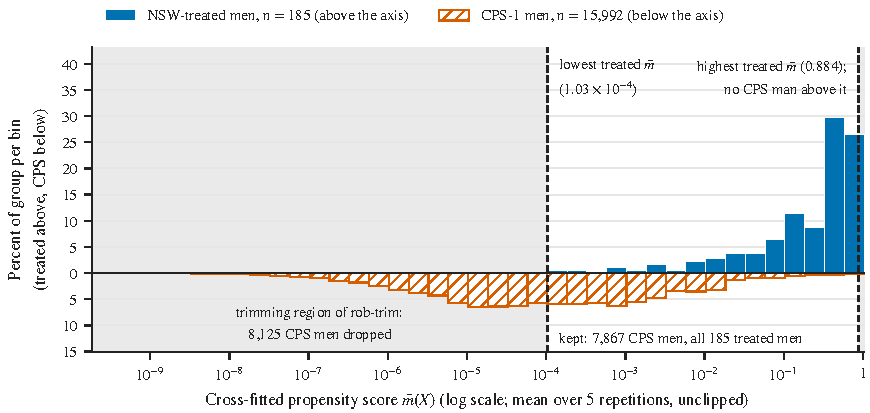
\includegraphics[width=0.8\textwidth]{figures/fig_overlap.pdf}
\caption{Overlap of the cross-fitted propensity score, NSW-treated men against CPS-1 men.
$\bar m(X)$ is the out-of-fold propensity of the primary specification (L2-penalized logit
on the 14-term basis $B(X)$, 5 folds $\times$ 5 repetitions), averaged over the repetitions
and unclipped. It was computed from covariates and treatment only, before the design gate.
The horizontal axis is $\log_{10} \bar m$. The bars show the percent of each group in each
bin of width 0.25 on the log scale: the $\PrimaryNTreated$ treated men above the axis (solid)
and the $\PrimaryNControl$ CPS men below it (hatched). The dashed lines mark the lowest and
highest treated $\bar m$; the shaded region outside them is the trimming region of
\run{rob-trim}, which drops the $\TrimNControlDropped$ CPS men in it, all below the lowest
treated value, and keeps $\TrimNControlKept$ CPS men and every treated man. The cutoff rests
on a single treated man's propensity, and the dropped men carry only
$\TrimDroppedWeightShare$\% of the control weight $\bar m/(1-\bar m)$. No treated man has
$\bar m > 0.9$ and no unit is clipped. The figure shows shares of units, not estimates, so it
has no error bars.}
\label{fig:overlap}
\end{figure}

\subsection{Hypotheses and decision rules}
\label{sec:rules}

All rules below were fixed before any outcome value was read.
\begin{description}
  \setlength{\itemsep}{2pt}
  \item[H1.] The ATT contrast on re78 is positive: H1 holds if and only if the 95\% interval
        of \run{main-aipw} lies entirely above zero. An interval that includes zero is never
        reported as ``no effect''. The result is worded as an effect only if H3 passes;
        otherwise it is a statistical contrast between the groups.
  \item[H3 (placebo).] The same estimator with outcome re75, conditioning on
        $X^{-} = X$ without re75 and u75 (bases of 11 and 8 terms), with the propensity
        refitted on $X^{-}$. H3 \emph{fails} if its 95\% interval excludes zero (this rule
        takes precedence); otherwise it \emph{passes} only if the whole interval lies within
        $[-900, 900]$ dollars (half the benchmark, fixed at the question gate); otherwise it
        is \emph{inconclusive}. A pass would be worded only as ``did not reject''. Two
        limits were stated in advance. A transitory dip in 1975 makes the placebo nonzero
        even if the assumption holds given re75. And because the placebo conditions on re74
        and u74, which for later-assigned treated men overlap 1975 and were used to select
        them, neither a pass nor a fail isolates confounding.
  \item[Disagreement rule.] If the H1 decision differs between \run{main-aipw} and any of
        \run{rob-trim}, covariate set (a), parametric nuisances or random-forest nuisances,
        the abstract says that the conclusion is not robust to that check. If covariate set
        (a) triggers, the sentence names what it drops: ``not robust to dropping race,
        ethnicity and degree status''. The Hajek IPW estimate triggers the same statement only
        if its point estimate lies outside the primary's 95\% interval, because its wider
        interval alone could change the decision. Checks that change the assumption or the
        estimand (covariate set (b), the OLS coefficient, the difference-in-differences
        estimate, the missing-outcome check) are reported but never trigger. The primary
        estimate is never replaced.
  \item[Sensitivity reading.] The shift that flips H1 is $t_0$, the distance from the
        nearer 95\% bound to zero. The paper reports the smallest equal-strength confounder
        that reaches $t_0$, names the benchmark covariate groups to which the conclusion is
        and is not robust, and always states the result for 1975 earnings
        (Section~\ref{sec:sensitivity}).
  \item[H2 (descriptive).] After the results gate only: the primary estimate minus
        the benchmark, with an approximate combined standard error. It is not a test, and
        closeness to the benchmark is never used to choose or rank estimators.
\end{description}

\section{Results: the main contrast (H1)}
\label{sec:results}

Table~\ref{tab:main}, panel A, and Figure~\ref{fig:forest} report the primary estimate. The
cross-fitted AIPW estimate of the ATT contrast is $\PrimaryEffect$ dollars, with standard
error $\PrimarySe$ and 95\% interval \ci{\PrimaryCiLow}{\PrimaryCiHigh} ($p = \PrimaryP$),
using all $\PrimaryN$ men. The treated men's mean 1978 earnings are $\PrimaryTreatedMean$
dollars, so the estimated counterfactual mean without the program is $\PrimaryCfMean$
dollars, and the contrast is $\PrimaryRelEffect$\% of it, with a delta-method interval of
\ci{\PrimaryRelCiLow\%}{\PrimaryRelCiHigh\%} that includes zero.

By the fixed rule H1 holds, because the 95\% interval lies entirely above zero. It holds by
$\PrimaryCiLow$ dollars, and that margin is smaller than the noise from the cross-fitting
splits. Table~\ref{tab:reps} shows the five repetitions that the design fixed. Their
estimates range from $\PrimaryThetaRepThree$ to $\PrimaryThetaRepFour$ dollars. Taken alone,
repetitions 0 and 1 have positive 95\% lower bounds, and the other
$\PrimaryNRepsCiIncludeZero$ give intervals that include zero. The primary estimate and the
H1 rule stay as fixed: the estimate is the mean over the five repetitions, and the decision
is the one that mean gives. But the positive decision is within cross-fitting noise, and
this paper does not call the contrast significant without saying so.

Because H3 failed (Section~\ref{sec:placebo}), the estimate is reported as a positive
statistical contrast between the NSW-treated men and reweighted CPS men under the stated
assumptions, not as an effect of the program.

\begin{table}[tbp]
\centering
\caption{The five cross-fitting repetitions of the primary estimate. Each repetition uses
seed $20261118 + s$ for its folds and inner cross-validation; the primary estimate is the
mean of the five, and its standard error includes the spread between them. The single-repetition
lower bounds, $\hat\theta_s - 1.96\,\widehat{\mathrm{SE}}_s$, are a post-results diagnostic
computed by run \run{post-results-derived} from \run{main-aipw}'s logged metrics
(Section~\ref{sec:deviations}). 1982 dollars.}
\label{tab:reps}
\small
\begin{tabular}{@{}l r r r@{}}
\toprule
Repetition & Estimate & SE & 95\% lower bound, this repetition alone \\
\midrule
$s = 0$ & $\PrimaryThetaRepZero$ & $\PrimarySeRepZero$ & $\PrimaryRepZeroCiLow$ \\
$s = 1$ & $\PrimaryThetaRepOne$ & $\PrimarySeRepOne$ & $\PrimaryRepOneCiLow$ \\
$s = 2$ & $\PrimaryThetaRepTwo$ & $\PrimarySeRepTwo$ & $\PrimaryRepTwoCiLow$ \\
$s = 3$ & $\PrimaryThetaRepThree$ & $\PrimarySeRepThree$ & $\PrimaryRepThreeCiLow$ \\
$s = 4$ & $\PrimaryThetaRepFour$ & $\PrimarySeRepFour$ & $\PrimaryRepFourCiLow$ \\
\midrule
Primary (mean, aggregated SE) & $\PrimaryEffect$ & $\PrimarySe$ & $\PrimaryCiLow$ \\
\bottomrule
\end{tabular}
\end{table}

\begin{table}[tbp]
\centering
\caption{Primary contrast (H1), placebo (H3), robustness estimates and the descriptive
comparison with the experimental benchmark (H2). 1982 dollars; 95\% confidence intervals.
Panel A: cross-fitted AIPW for the ATT on 1978 earnings, with an L2-logit propensity on
$B(X)$ and a gradient-boosted control outcome model, 5 folds $\times$ 5 repetitions and
influence-function standard errors (SE $\PrimarySe$); $n = \PrimaryN$. By the fixed rule H1
holds, because the interval lies above zero, but only just: $\PrimaryNRepsCiIncludeZero$ of
the 5 single-repetition intervals include zero, so the decision lies within cross-fitting
noise. Because H3 failed, the estimate is a statistical contrast between the groups, not an
effect of the program. Panel B: the same estimator with outcome re75, conditioning on the
covariates without re75 and u75 (SE $\PlaceboSe$). The interval excludes zero, so H3 fails.
The failure is consistent with the pre-program earnings dip and with the different meaning
of re74 in the two groups, so it is not proof of bias in panel A. Panel C: every planned
robustness estimate; the primary estimate is never replaced. Panel D: the primary estimate
minus the benchmark of \citet[Table~3]{dehejia1999}, descriptive only.
$^{a}$~A row that can trigger the disagreement rule triggers when its H1 decision differs
from panel A's; each ``Triggered'' cell is the run's own logged flag, and ``--'' marks rows
that change the assumption or the estimand and never trigger.
$^{b}$~Drops the $\TrimNControlDropped$ CPS men whose $\bar m$ lies outside the treated
men's range, keeps $\TrimNControlKept$ and every treated man, and re-fits the nuisance
models on the kept men. The dropped men carry $\TrimDroppedWeightShare$\% of the control
weight, so the check does not test reliance on them.
$^{c}$~Set (a) conditions on age, educ, married, re74, re75, u74 and u75, so it drops black,
hisp and nodegree. Set (b) drops re74 and u74, which are measured over different months for
treated and CPS men.
$^{d}$~The Hajek IPW row (bootstrap SE $\IpwSe$) triggers only if its point estimate lies
outside panel A's 95\% interval.
$^{e}$~A different estimand and assumption: the ATT on re78 $-$ re74 under conditional
parallel trends given the time-invariant covariates.
$^{f}$~The difference $\pm 1.96$ times a combined SE of $\HTwoSeCombined$,
$\sqrt{\mathrm{SE}^2 + \HTwoBenchmarkSe^2}$, which ignores the positive covariance from the
$\PrimaryNTreated$ treated men the two estimates share, so it overstates the uncertainty.}
\label{tab:main}
\footnotesize
\setlength{\tabcolsep}{4pt}
\resizebox{\textwidth}{!}{% Generated by code/tab_main.py from logged runs. Do not edit by hand; rerun the script.
% Needs \usepackage{booktabs,icomma} and % Generated by `crew.py numbers` from claims.jsonl. Do not edit by hand.
% Each macro is a number taken from a logged run; see claims.jsonl.
\newcommand{\PrimaryEffect}{1,573}  % primary-effect
\newcommand{\PrimaryCiLow}{9.6}  % primary-ci-low
\newcommand{\PrimaryCiHigh}{3,136}  % primary-ci-high
\newcommand{\PrimarySe}{798}  % primary-se
\newcommand{\PrimaryP}{0.049}  % primary-p
\newcommand{\PrimaryN}{16,177}  % primary-n
\newcommand{\PrimaryNTreated}{185}  % primary-n-treated
\newcommand{\PrimaryNControl}{15,992}  % primary-n-control
\newcommand{\PrimaryNClipped}{0}  % primary-n-clipped
\newcommand{\PrimaryTreatedMean}{6,349}  % primary-treated-mean
\newcommand{\PrimaryCfMean}{4,776}  % primary-cf-mean
\newcommand{\PrimaryControlMeanRaw}{14,847}  % primary-control-mean-raw
\newcommand{\PrimaryRelEffect}{32.9}  % primary-rel-effect
\newcommand{\PrimaryRelCiLow}{-5.1}  % primary-rel-ci-low
\newcommand{\PrimaryRelCiHigh}{71.0}  % primary-rel-ci-high
\newcommand{\PrimaryReSeventyeightInvalidTreated}{0}  % primary-re78-invalid-treated
\newcommand{\PrimaryReSeventyeightInvalidControl}{0}  % primary-re78-invalid-control
\newcommand{\OverlapTreatedAbovePointnine}{0.000}  % overlap-treated-above-09
\newcommand{\OverlapKishEss}{126.4}  % overlap-kish-ess
\newcommand{\OverlapMaxControlWeight}{6.41}  % overlap-max-control-weight
\newcommand{\OverlapMbarMaxDiff}{5.0e-13}  % overlap-mbar-max-diff
\newcommand{\PrimaryThetaRepZero}{1,597}  % primary-theta-rep0
\newcommand{\PrimarySeRepZero}{786}  % primary-se-rep0
\newcommand{\PrimaryThetaRepOne}{1,612}  % primary-theta-rep1
\newcommand{\PrimarySeRepOne}{794}  % primary-se-rep1
\newcommand{\PrimaryThetaRepTwo}{1,522}  % primary-theta-rep2
\newcommand{\PrimarySeRepTwo}{787}  % primary-se-rep2
\newcommand{\PrimaryThetaRepThree}{1,511}  % primary-theta-rep3
\newcommand{\PrimarySeRepThree}{784}  % primary-se-rep3
\newcommand{\PrimaryThetaRepFour}{1,621}  % primary-theta-rep4
\newcommand{\PrimarySeRepFour}{828}  % primary-se-rep4
\newcommand{\PrimaryRepZeroCiLow}{55.2}  % primary-rep0-ci-low
\newcommand{\PrimaryRepOneCiLow}{56.5}  % primary-rep1-ci-low
\newcommand{\PrimaryRepTwoCiLow}{-20.1}  % primary-rep2-ci-low
\newcommand{\PrimaryRepThreeCiLow}{-26.0}  % primary-rep3-ci-low
\newcommand{\PrimaryRepFourCiLow}{-2.6}  % primary-rep4-ci-low
\newcommand{\PrimaryNRepsCiIncludeZero}{3}  % primary-n-reps-ci-include-zero
\newcommand{\PlaceboEffect}{-1,543}  % placebo-effect
\newcommand{\PlaceboCpsReSeventyfiveTopcoded}{3,007}  % placebo-cps-re75-topcoded
\newcommand{\PlaceboSe}{590}  % placebo-se
\newcommand{\PlaceboCiLow}{-2,699}  % placebo-ci-low
\newcommand{\PlaceboCiHigh}{-387}  % placebo-ci-high
\newcommand{\PlaceboP}{0.009}  % placebo-p
\newcommand{\PlaceboVerdict}{-1}  % placebo-verdict
\newcommand{\PlaceboNClipped}{0}  % placebo-n-clipped
\newcommand{\PlaceboSeNeeded}{459}  % placebo-se-needed
\newcommand{\TrimEffect}{1,514}  % trim-effect
\newcommand{\TrimCiLow}{-80}  % trim-ci-low
\newcommand{\TrimCiHigh}{3,107}  % trim-ci-high
\newcommand{\TrimNControlKept}{7,867}  % trim-n-control-kept
\newcommand{\TrimNControlDropped}{8,125}  % trim-n-control-dropped
\newcommand{\TrimThetaRepZero}{1,608}  % trim-theta-rep0
\newcommand{\TrimThetaRepOne}{1,265}  % trim-theta-rep1
\newcommand{\TrimThetaRepTwo}{1,624}  % trim-theta-rep2
\newcommand{\TrimThetaRepThree}{1,613}  % trim-theta-rep3
\newcommand{\TrimThetaRepFour}{1,458}  % trim-theta-rep4
\newcommand{\CovsetAEffect}{1,081}  % covset-a-effect
\newcommand{\CovsetACiLow}{-183}  % covset-a-ci-low
\newcommand{\CovsetACiHigh}{2,346}  % covset-a-ci-high
\newcommand{\CovsetBEffect}{1,213}  % covset-b-effect
\newcommand{\CovsetBCiLow}{-247}  % covset-b-ci-low
\newcommand{\CovsetBCiHigh}{2,673}  % covset-b-ci-high
\newcommand{\LearnerLinearEffect}{1,433}  % learner-linear-effect
\newcommand{\LearnerLinearCiLow}{-88}  % learner-linear-ci-low
\newcommand{\LearnerLinearCiHigh}{2,953}  % learner-linear-ci-high
\newcommand{\LearnerRfEffect}{1,584}  % learner-rf-effect
\newcommand{\LearnerRfCiLow}{144}  % learner-rf-ci-low
\newcommand{\LearnerRfCiHigh}{3,025}  % learner-rf-ci-high
\newcommand{\OlsCoef}{1,199}  % ols-coef
\newcommand{\OlsCiLow}{-28}  % ols-ci-low
\newcommand{\OlsCiHigh}{2,426}  % ols-ci-high
\newcommand{\IpwEffect}{1,453}  % ipw-effect
\newcommand{\IpwSe}{728}  % ipw-se
\newcommand{\IpwCiLow}{26}  % ipw-ci-low
\newcommand{\IpwCiHigh}{2,879}  % ipw-ci-high
\newcommand{\DiffSeventyfourEffect}{2,798}  % diff74-effect
\newcommand{\DiffSeventyfourCiLow}{1,331}  % diff74-ci-low
\newcommand{\DiffSeventyfourCiHigh}{4,265}  % diff74-ci-high
\newcommand{\TrimMinusMain}{-59}  % trim-minus-main
\newcommand{\TrimRepMin}{1,265}  % trim-rep-min
\newcommand{\TrimRepMax}{1,624}  % trim-rep-max
\newcommand{\TrimDroppedWeightShare}{0.09}  % trim-dropped-weight-share
\newcommand{\SensTauZerozero}{1,199}  % sens-tau00
\newcommand{\SensTargetZero}{9.6}  % sens-target-zero
\newcommand{\SensRsqZero}{0.0011}  % sens-r2-zero
\newcommand{\SensSigmaZero}{6,987}  % sens-sigma0
\newcommand{\SensBenchAgeRsqd}{0.535}  % sens-bench-age-r2d
\newcommand{\SensBenchAgeRsqy}{0.0159}  % sens-bench-age-r2y
\newcommand{\SensBenchAgeBias}{785}  % sens-bench-age-bias
\newcommand{\SensBenchEducRsqd}{0.292}  % sens-bench-educ-r2d
\newcommand{\SensBenchEducRsqy}{0.0026}  % sens-bench-educ-r2y
\newcommand{\SensBenchEducBias}{239}  % sens-bench-educ-bias
\newcommand{\SensBenchBlackRsqd}{0.000}  % sens-bench-black-r2d
\newcommand{\SensBenchBlackRsqy}{0.0008}  % sens-bench-black-r2y
\newcommand{\SensBenchBlackBias}{0}  % sens-bench-black-bias
\newcommand{\SensBenchHispRsqd}{0.086}  % sens-bench-hisp-r2d
\newcommand{\SensBenchHispRsqy}{0.0001}  % sens-bench-hisp-r2y
\newcommand{\SensBenchHispBias}{24}  % sens-bench-hisp-bias
\newcommand{\SensBenchMarriedRsqd}{0.000}  % sens-bench-married-r2d
\newcommand{\SensBenchMarriedRsqy}{0.0002}  % sens-bench-married-r2y
\newcommand{\SensBenchMarriedBias}{0}  % sens-bench-married-bias
\newcommand{\SensBenchNodegreeRsqd}{0.000}  % sens-bench-nodegree-r2d
\newcommand{\SensBenchNodegreeRsqy}{0.0001}  % sens-bench-nodegree-r2y
\newcommand{\SensBenchNodegreeBias}{0}  % sens-bench-nodegree-bias
\newcommand{\SensBenchEarnSeventyfourRsqd}{0.185}  % sens-bench-earn74-r2d
\newcommand{\SensBenchEarnSeventyfourRsqy}{0.0345}  % sens-bench-earn74-r2y
\newcommand{\SensBenchEarnSeventyfourBias}{699}  % sens-bench-earn74-bias
\newcommand{\SensBenchEarnSeventyfiveRsqd}{0.532}  % sens-bench-earn75-r2d
\newcommand{\SensBenchEarnSeventyfiveRsqy}{0.0868}  % sens-bench-earn75-r2y
\newcommand{\SensBenchEarnSeventyfiveBias}{1,876}  % sens-bench-earn75-bias
\newcommand{\HTwoDiff}{-221}  % h2-diff
\newcommand{\HTwoSeCombined}{1,018}  % h2-se-combined
\newcommand{\HTwoCiLow}{-2,217}  % h2-ci-low
\newcommand{\HTwoCiHigh}{1,774}  % h2-ci-high
\newcommand{\HTwoBenchmarkValue}{1,794}  % h2-benchmark-value
\newcommand{\HTwoBenchmarkSe}{633}  % h2-benchmark-se
 for the macros
% (icomma keeps the thousands comma in math mode, e.g. $1,573$, without a space).
\begin{tabular}{@{}l r c c c@{}}
\toprule
 & & & \multicolumn{2}{c}{Disagreement rule$^{a}$} \\
\cmidrule(l){4-5}
Specification & Estimate & 95\% CI & Can trigger & Triggered \\
\midrule
\multicolumn{5}{@{}l}{\emph{A. Primary (H1): ATT contrast on 1978 earnings, all $\PrimaryNTreated$ treated men}} \\
% main-aipw: effect = 1572.764316543202, ci_low = 9.60806603853689, ci_high = 3135.9205670478673, h1_holds = True
Cross-fitted AIPW, ten covariates & ${\PrimaryEffect}$ & [${\PrimaryCiLow}$, ${\PrimaryCiHigh}$] & \multicolumn{2}{c}{reference} \\
\midrule
\multicolumn{5}{@{}l}{\emph{B. Placebo (H3): same estimator, outcome 1975 earnings, without re75 and u75}} \\
% placebo-re75: effect = -1542.6727678455577, ci_low = -2698.703587936461, ci_high = -386.6419477546542, verdict = 'fail', ci_excludes_zero = True
Placebo on re75 & ${\PlaceboEffect}$ & [${\PlaceboCiLow}$, ${\PlaceboCiHigh}$] & \multicolumn{2}{c}{H3: fail (CI excludes 0)} \\
\midrule
\multicolumn{5}{@{}l}{\emph{C. Robustness, outcome 1978 earnings (all reported; the primary is never replaced)}} \\
% rob-trim: effect = 1513.633290127726, ci_low = -79.74415537175878, ci_high = 3107.010735627211, triggers_abstract_statement = True
Control-only trimming$^{b}$ & ${\TrimEffect}$ & [${\TrimCiLow}$, ${\TrimCiHigh}$] & yes & yes \\
% rob-learners: linear_effect = 1432.826452439745, linear_ci_low = -87.7452885343896, linear_ci_high = 2953.3981934138797, linear_triggers_abstract_statement = True
Learners (a): parametric nuisances & ${\LearnerLinearEffect}$ & [${\LearnerLinearCiLow}$, ${\LearnerLinearCiHigh}$] & yes & yes \\
% rob-learners: rf_effect = 1584.3206098522835, rf_ci_low = 143.53041989291546, rf_ci_high = 3025.1107998116513, rf_triggers_abstract_statement = False
Learners (b): random forests & ${\LearnerRfEffect}$ & [${\LearnerRfCiLow}$, ${\LearnerRfCiHigh}$] & yes & no \\
% rob-covsets: covset_a_effect = 1081.412122525752, covset_a_ci_low = -182.92188343331668, covset_a_ci_high = 2345.7461284848205, covset_a_triggers_abstract_statement = True
Covariate set (a): earnings-history core$^{c}$ & ${\CovsetAEffect}$ & [${\CovsetACiLow}$, ${\CovsetACiHigh}$] & yes & yes \\
% rob-covsets: covset_b_effect = 1213.0263587652248, covset_b_ci_low = -247.15769865761308, covset_b_ci_high = 2673.2104161880625
Covariate set (b): single lag$^{c}$ & ${\CovsetBEffect}$ & [${\CovsetBCiLow}$, ${\CovsetBCiHigh}$] & no & -- \\
% rob-estimators: ols_effect = 1198.9873005075867, ols_ci_low = -28.29833050947059, ols_ci_high = 2426.2729315246443
OLS coefficient on treat (HC2) & ${\OlsCoef}$ & [${\OlsCiLow}$, ${\OlsCiHigh}$] & no & -- \\
% rob-estimators: ipw_effect = 1452.6422941153287, ipw_ci_low = 26.368583140310875, ipw_ci_high = 2878.9160050903465, ipw_triggers_abstract_statement = False
Hajek IPW (bootstrap SE) & ${\IpwEffect}$ & [${\IpwCiLow}$, ${\IpwCiHigh}$] & yes$^{d}$ & no \\
% rob-diff74: effect = 2797.7925471618755, ci_low = 1330.8635691492887, ci_high = 4264.721525174462, triggers_abstract_statement = False
Conditional DiD on re78 $-$ re74$^{e}$ & ${\DiffSeventyfourEffect}$ & [${\DiffSeventyfourCiLow}$, ${\DiffSeventyfourCiHigh}$] & no & -- \\
\midrule
\multicolumn{5}{@{}l}{\emph{D. H2, descriptive: primary minus the experimental benchmark}} \\
% h2-benchmark: benchmark = 1794.0, benchmark_se = 633.0, h2_diff = -221.23568345679791, h2_se_combined = 1018.21628447082, h2_ci_low = -2216.9029294917955, h2_ci_high = 1774.4315625781996
Primary $-$ ${\HTwoBenchmarkValue}$ (SE ${\HTwoBenchmarkSe}$) & ${\HTwoDiff}$ & [${\HTwoCiLow}$, ${\HTwoCiHigh}$]$^{f}$ & \multicolumn{2}{c}{no test} \\
\bottomrule
\end{tabular}
}
\end{table}

\section{The placebo check (H3) and what its failure means}
\label{sec:placebo}

Panel B of Table~\ref{tab:main} and panel (b) of Figure~\ref{fig:forest} report the placebo.
Applied to 1975 earnings, without conditioning on re75 or u75, the same estimator gives
$\PlaceboEffect$ dollars (SE $\PlaceboSe$; 95\% interval
\ci{\PlaceboCiLow}{\PlaceboCiHigh}; $p = \PlaceboP$), with $\PlaceboNClipped$ clipped units.
The interval excludes zero, so H3 fails by the rule that takes precedence. Given their 1974
earnings history and demographics, the treated men earned less in 1975 than comparable CPS
men. Under the rule fixed at the question gate, H1 is therefore worded as a statistical
contrast between the groups, never as an effect of the program.

H3 could not have passed in any case. A pass needs the whole interval inside $[-900, 900]$,
which is possible even at a zero estimate only if the placebo's standard error is below
$\PlaceboSeNeeded$ dollars. The realized standard error is $\PlaceboSe$, so H3 could only
fail or be inconclusive. The design anticipated this possibility and kept the bound.

The failure is a statistical contrast between the groups in 1975, not an effect of the
program, which had not yet begun, and it is not proof that the primary estimate is biased.
Three features of the data, all stated before the placebo ran, can produce it.
\begin{itemize}
  \setlength{\itemsep}{1pt}
  \item \textbf{The pre-program dip.} If the treated men's 1975 earnings were transitorily
        depressed, the placebo is
        negative even if unconfoundedness holds given re75, because the primary analysis
        conditions on re75 and the placebo does not.
  \item \textbf{The re74 caveat.} The placebo conditions on re74 and u74. For treated men
        assigned later in the experiment, ``re74'' covers months that largely overlap 1975,
        and men assigned after April 1976 were admitted only if it was zero. The conditioning
        set is thus linked to the outcome for treated men only, by definition and by sample
        selection.
  \item \textbf{Top-coding.} The placebo outcome re75 is top-coded for CPS men
        ($\PlaceboCpsReSeventyfiveTopcoded$ at the maximum) and not for NSW men.
\end{itemize}
A failure is what the literature led the crew to expect: \citet{imbens2025} report large,
negative and significant placebo estimates on 1975 earnings for every non-experimental
estimator on this sample, and \citet{imbens2015} reports pseudo-outcome tests that reject.
The failure does not tell us whether the primary contrast is biased. It does mean the data
give no licence to read the contrast as the program's effect.

\begin{figure}[tbp]
\centering
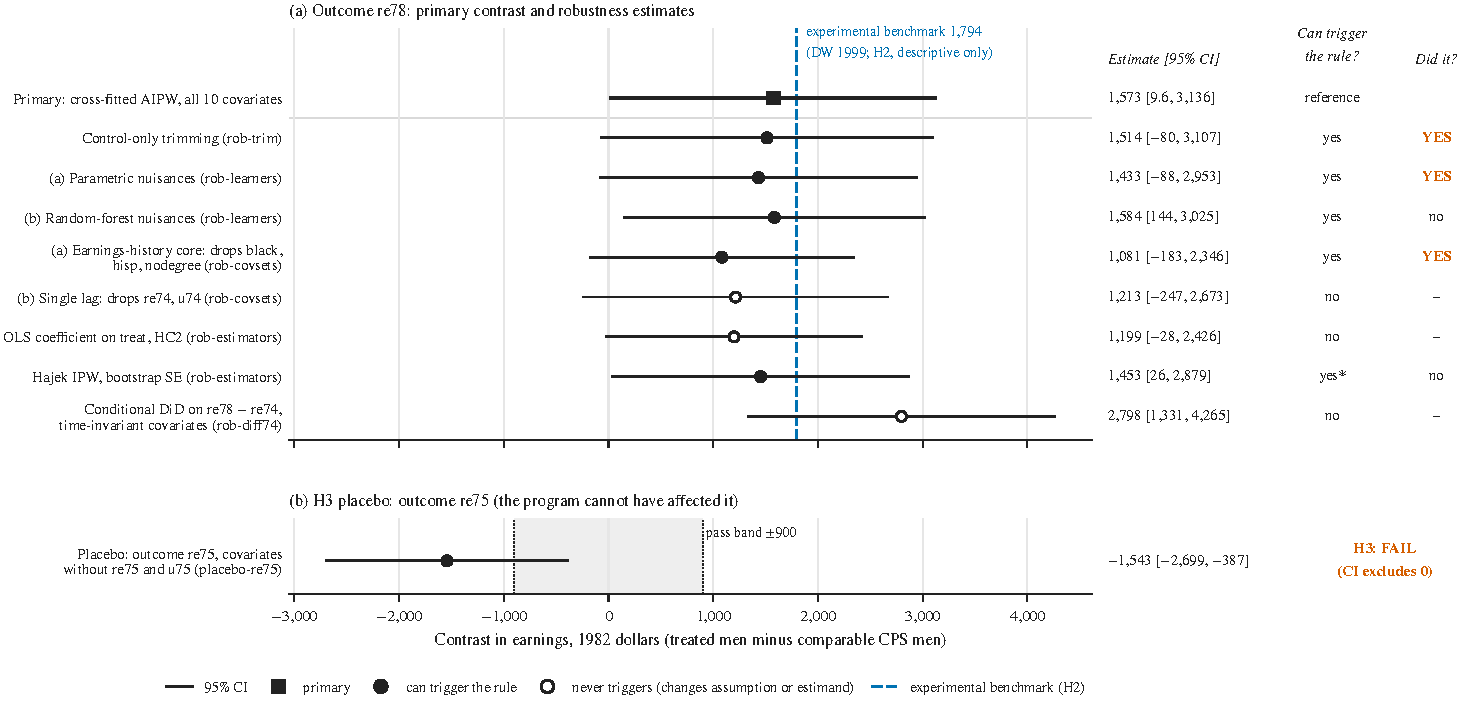
\includegraphics[width=\textwidth]{figures/fig_forest.pdf}
\caption{The primary contrast, every planned robustness estimate and the H3 placebo, each
with its 95\% confidence interval. Panel (a), outcome 1978 earnings: the primary estimate
(square) is the cross-fitted AIPW ATT contrast, $\PrimaryEffect$ (SE $\PrimarySe$, 95\% CI
\ci{\PrimaryCiLow}{\PrimaryCiHigh}), over all $\PrimaryNTreated$ treated men. Because the
placebo failed (panel b), this is a statistical contrast, not an effect of the program, and
its lower bound lies within cross-fitting noise of zero. The rows below are in the order of
the analysis plan. ``Can trigger'' says whether the row can trigger the disagreement rule,
fixed before any outcome was read; ``Did it?'' is the run's logged flag. Control-only
trimming, parametric nuisances and covariate set (a), which drops race, ethnicity and
degree status, trigger; the random-forest row does not; the Hajek IPW row (yes*) could
trigger only if its point estimate lay outside the primary's 95\% CI, and it does not. Filled
dots can trigger the rule. Open dots change the conditioning set, the estimator or the
estimand and never trigger: covariate set (b), the OLS coefficient and the conditional
difference-in-differences contrast on re78 $-$ re74. The dashed blue line is the
experimental benchmark of $\HTwoBenchmarkValue$ dollars \citep{dehejia1999}, drawn for
reference only (H2, descriptive); no row is compared with it, ranked by it or chosen by it.
Panel (b), outcome 1975 earnings (the H3 placebo): the same estimator, conditioning on the
covariates without re75 and u75, gives $\PlaceboEffect$ (SE $\PlaceboSe$, 95\% CI
\ci{\PlaceboCiLow}{\PlaceboCiHigh}). The interval excludes zero, so H3 fails. The gray band is
the pass band of $\pm 900$ dollars. Standard errors are influence-function based for the
AIPW rows, HC2 for OLS and a 999-draw bootstrap for the Hajek IPW. $n = \PrimaryN$ in every
row except control-only trimming, which keeps $\TrimNControlKept$ CPS men and all treated
men. 1982 dollars.}
\label{fig:forest}
\end{figure}

\section{Robustness and the disagreement rule}
\label{sec:robustness}

Panel C of Table~\ref{tab:main} reports every planned robustness estimate. Each was run once,
in the planned order, after the design gate. Each point estimate is positive. What differs
is whether the 95\% interval excludes zero, and so whether the H1 decision agrees with the
primary's.

\paragraph{Checks that can trigger the disagreement rule.}
\begin{itemize}
  \setlength{\itemsep}{1pt}
  \item \textbf{Control-only trimming} (\run{rob-trim}) gives $\TrimEffect$
        \ci{\TrimCiLow}{\TrimCiHigh}, after dropping $\TrimNControlDropped$ CPS men and
        keeping $\TrimNControlKept$. Its interval includes zero, so it \emph{triggers} the
        rule. What the check measures matters for how to read this. It re-fits the nuisance
        models on the kept CPS men; it does not test reliance on the dropped men, who carry
        only $\TrimDroppedWeightShare$\% of the control weight, and its cutoff rests on one
        treated man's propensity. Trimming moves the estimate by $\TrimMinusMain$ dollars,
        less than the spread of its own five repetitions (from $\TrimRepMin$ to $\TrimRepMax$
        dollars). The trigger is therefore consistent with cross-fitting and refitting
        noise near a lower bound just above zero, not with an overlap failure.
  \item \textbf{Parametric nuisances} (an L2 logit propensity and an OLS outcome model on
        $B(X)$) give $\LearnerLinearEffect$ \ci{\LearnerLinearCiLow}{\LearnerLinearCiHigh};
        the interval includes zero, so this check \emph{triggers}.
  \item \textbf{Random-forest nuisances} (500 trees, at least 5 men per leaf) give
        $\LearnerRfEffect$ \ci{\LearnerRfCiLow}{\LearnerRfCiHigh}; the interval lies above
        zero, so this check does not trigger.
  \item \textbf{Covariate set (a)}, the earnings-history core (age, educ, married, re74,
        re75, u74, u75), gives $\CovsetAEffect$ \ci{\CovsetACiLow}{\CovsetACiHigh}; it
        \emph{triggers}. This set leaves out black, hisp and nodegree, and black has the
        largest raw imbalance of any covariate (Table~\ref{tab:summary}). The check
        therefore asks whether the conclusion survives without conditioning on race,
        ethnicity and degree status, not only whether it is fragile to the covariate set,
        and the abstract names what it drops.
  \item \textbf{Hajek IPW}, a normalized inverse-probability-weighted ATT with a
        999-draw bootstrap standard error of $\IpwSe$, gives $\IpwEffect$
        \ci{\IpwCiLow}{\IpwCiHigh}. Its point estimate lies inside the primary's interval, so
        it does not trigger.
\end{itemize}
Three of the four checks that can trigger the rule through the H1 decision do so. By the fixed rule, the
conclusion is not robust to control-only trimming, to dropping race, ethnicity and degree
status, or to parametric nuisance models, and the abstract says so.

\paragraph{Checks that never trigger.} These change the conditioning set, the estimand or
the assumption. Covariate set (b), which drops re74 and u74, the covariate measured over
different months in the two groups, gives $\CovsetBEffect$ \ci{\CovsetBCiLow}{\CovsetBCiHigh}.
The OLS coefficient on treatment with $B(X)$ controls and HC2 standard errors, a regression
coefficient and not an ATT, is $\OlsCoef$ \ci{\OlsCiLow}{\OlsCiHigh}. Both intervals include
zero. The conditional difference-in-differences estimate on $\var{re78} - \var{re74}$, given
the time-invariant covariates only, is $\DiffSeventyfourEffect$
\ci{\DiffSeventyfourCiLow}{\DiffSeventyfourCiHigh}. It rests on conditional parallel trends
from each group's recorded ``re74'' base period to 1978, which is not the same calendar base
in the two groups. The design stated in advance that this estimate is biased upward if the
treated men's base earnings were already transitorily depressed, more so for later
assignees, and downward if their lower earnings reflect a permanently lower growth path. It
is reported as an estimate under a different assumption, not as a defence of the primary.

\paragraph{The missing-outcome check} (inverse-probability-of-observation weighting) was
not run. Its trigger, a between-arm gap above 0.02 in the share of missing or inadmissible
re78 values, did not fire: no value is missing or inadmissible in either arm.

\section{Sensitivity to an unobserved confounder}
\label{sec:sensitivity}

The sensitivity analysis is the parametric model with a binary unobserved confounder
specified in the adopted design. $U \sim \text{Bernoulli}(0.5)$ is independent of $X$; the
participation equation is $\operatorname{logit} P(D = 1 \mid X, U) = \gamma' B(X) + \alpha U$
and the outcome equation is $\var{re78} = \tau D + \beta' B(X) + \delta U + \varepsilon$,
$\varepsilon \sim N(0, \sigma^2)$, with a constant treatment coefficient. The model is fitted
by EM for fixed $(\alpha, \delta)$. The strength of $U$ is expressed as $R^2_D$, the share of
the residual latent variance of participation it explains, and $R^2_Y$, the share of the
residual variance of re78 it explains. The bias $\tau(\alpha, \delta) - \tau(0, 0)$ is
computed within this model and applied additively to the AIPW estimate, as an
approximation. The model's own $U$-free estimate is $\tau(0, 0) = \SensTauZerozero$ dollars,
equal to the OLS coefficient, against the AIPW estimate of $\PrimaryEffect$; the residual SD
of re78 in the OLS fit is $\SensSigmaZero$ dollars.

The target is $t_0 = \SensTargetZero$ dollars: the shift that moves the lower 95\% bound to
zero and so reverses the H1 decision. It is tiny because the lower bound sits just above
zero. On the diagonal $R^2_D = R^2_Y$, the smallest confounder whose bias reaches $t_0$ has
$R^2_{*,0} = \SensRsqZero$. A confounder this weak, explaining that share of the residual
variance in both equations, would reverse the decision.

Each benchmark places a covariate group at the strength that dropping it from $B(X)$
implies, and fits the model there (Table~\ref{tab:sens}, Figure~\ref{fig:sens}). The
conclusion is not robust to a confounder as strong as the 1975 earnings group: at that
strength $|\text{bias}|$ is $\SensBenchEarnSeventyfiveBias$ dollars, larger than the point
estimate itself. The positive contrast could therefore be produced by unobserved selection
of that strength, for example an unobserved 1976 earnings shock, which is plausibly at least
as strongly related to participation as the 1975 shock. The conclusion is also not robust
to confounders as strong as age, education, hispanic or the 1974 earnings group (the
last measured over different periods in the two groups).

The rule's ``robust'' verdicts for black, married and nodegree carry no information. For
these three groups the treatment-side benchmark $R^2_D$ is floored at zero: by the benchmark
formula, a zero means that dropping the group did not lower the variance of the fitted logit
index. Their small $|\text{bias}|$ values reflect the floor, not the strength of race,
marital status or degree as confounders, and the paper does not describe the conclusion as
robust to a confounder as strong as any of them. Race is the covariate with the largest raw
imbalance. No benchmark group therefore gives evidence of robustness, and the weakest
informative benchmark, hispanic, is already strong enough to reverse the decision.

\begin{table}[tbp]
\centering
\caption{Sensitivity benchmarks: covariate groups placed at the strength that dropping them
from $B(X)$ implies, in the binary-confounder model of the adopted design (run
\run{sens-imbens}). $|\text{bias}|$ is the larger of the two signs of $U$'s outcome
coefficient, from the EM fit at that point, in 1982 dollars. The verdict compares
$|\text{bias}|$ with $t_0 = \SensTargetZero$ dollars, the shift that reverses the H1
decision. The groups marked ``no information'' have $R^2_D$ floored at zero, so the rule's
``robust'' verdict for them is an artifact of the floor. The bias is applied additively to
the AIPW estimate as an approximation.}
\label{tab:sens}
\small
\begin{tabular}{@{}l l r r r l@{}}
\toprule
Group & Terms dropped & $R^2_D$ & $R^2_Y$ & $|\text{bias}|$ & Verdict \\
\midrule
age & age, age$^2$ & $\SensBenchAgeRsqd$ & $\SensBenchAgeRsqy$ & $\SensBenchAgeBias$ & not robust \\
educ & educ, educ$^2$ & $\SensBenchEducRsqd$ & $\SensBenchEducRsqy$ & $\SensBenchEducBias$ & not robust \\
black & black & $\SensBenchBlackRsqd$ & $\SensBenchBlackRsqy$ & $\SensBenchBlackBias$ & no information \\
hisp & hisp & $\SensBenchHispRsqd$ & $\SensBenchHispRsqy$ & $\SensBenchHispBias$ & not robust \\
married & married & $\SensBenchMarriedRsqd$ & $\SensBenchMarriedRsqy$ & $\SensBenchMarriedBias$ & no information \\
nodegree & nodegree & $\SensBenchNodegreeRsqd$ & $\SensBenchNodegreeRsqy$ & $\SensBenchNodegreeBias$ & no information \\
earnings74 & re74, re74$^2$, u74 & $\SensBenchEarnSeventyfourRsqd$ & $\SensBenchEarnSeventyfourRsqy$ & $\SensBenchEarnSeventyfourBias$ & not robust \\
earnings75 & re75, re75$^2$, u75 & $\SensBenchEarnSeventyfiveRsqd$ & $\SensBenchEarnSeventyfiveRsqy$ & $\SensBenchEarnSeventyfiveBias$ & not robust \\
\bottomrule
\end{tabular}
\end{table}

\begin{figure}[tbp]
\centering
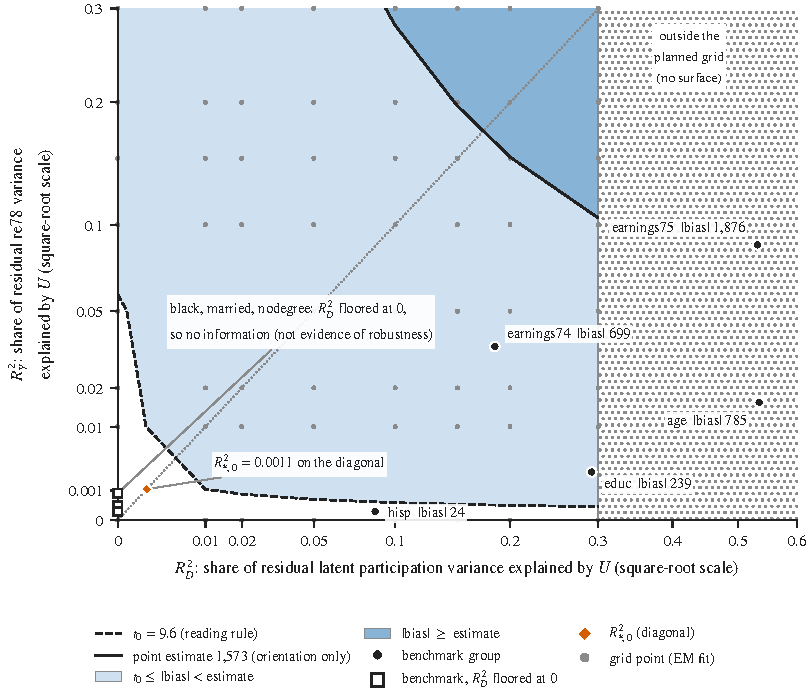
\includegraphics[width=0.72\textwidth]{figures/fig_sensitivity.pdf}
\caption{Sensitivity of the primary contrast to an unobserved binary confounder $U$ (run
\run{sens-imbens}). The horizontal axis is $R^2_D$, the share of the residual latent variance
of participation that $U$ explains; the vertical axis is $R^2_Y$, the share of the residual
variance of re78 that $U$ explains. Both axes use a square-root scale. The shading and
contour lines show the larger $|\text{bias}|$ of the two signs of $U$'s outcome coefficient,
from the EM fits on the planned grid (gray dots), interpolated linearly. The dashed line is
the target $t_0 = \SensTargetZero$ dollars, the shift that reverses the H1 decision; the solid
line, at the point estimate $\PrimaryEffect$, is drawn for orientation only. The orange
diamond is the diagonal breakdown point $R^2_{*,0} = \SensRsqZero$. The dots are the
benchmark covariate groups, labelled with the $|\text{bias}|$ of the EM fit at that point,
which is what the reading rule uses; the interpolated surface is coarse near the axes, and
hispanic lies below the interpolated $t_0$ line although its fitted $|\text{bias}|$,
$\SensBenchHispBias$ dollars, exceeds $t_0$. The open squares on the vertical axis are black,
married and nodegree, whose $R^2_D$ is floored at zero; their ``robust'' verdicts carry no
information. Age and earnings75 have $R^2_D$ above the grid's 0.30, so the horizontal axis
extends past the grid, and the hatched region has no surface. The bias is computed within the
parametric model and transferred additively to the AIPW estimate as an approximation.
$n = \PrimaryN$.}
\label{fig:sens}
\end{figure}

\section{Comparison with the experimental benchmark (H2, descriptive)}
\label{sec:h2}

After the results gate, run \run{h2-benchmark} computed the primary estimate minus the
experimental benchmark of $\HTwoBenchmarkValue$ dollars (SE $\HTwoBenchmarkSe$;
\citealp[Table~3]{dehejia1999}). The difference is $\HTwoDiff$ dollars, with an approximate
combined standard error of $\HTwoSeCombined$ and a descriptive band of
\ci{\HTwoCiLow}{\HTwoCiHigh} (Table~\ref{tab:main}, panel D). The combined standard error,
$\sqrt{\mathrm{SE}^2 + \HTwoBenchmarkSe^2}$, ignores the positive covariance that comes from
the $\PrimaryNTreated$ treated men the two estimates share, so it overstates the uncertainty
and the band is too wide.

This is a description, not a test, and it carries no verdict. Closeness to the benchmark was
never used to choose, rank or adjust any estimator, and no file written before the results
gate compares any estimate with it. Nor is closeness evidence that the identifying assumption
holds: the placebo failed, and \citet{imbens2025} find that estimates near the benchmark and
failed placebo tests coexist on this sample. The two estimates also differ in kind. The
benchmark is an experimental estimate of the program's effect; the primary estimate is a
statistical contrast with reweighted CPS men.

\section{Limitations}
\label{sec:limitations}

\begin{itemize}
  \setlength{\itemsep}{1pt}
  \item \textbf{No causal reading.} The placebo failed, so the main result is a contrast
        between groups. The data cannot tell whether the failure reflects confounding, the
        pre-program dip, the re74 measurement difference or top-coding.
  \item \textbf{A decision at the edge.} The H1 decision depends on a lower bound of
        $\PrimaryCiLow$ dollars, within cross-fitting noise; three of four triggering checks
        and every informative sensitivity benchmark reverse it.
  \item \textbf{Measurement differs by group.} CPS earnings are top-coded administrative
        records and NSW earnings are survey reports, for the outcome and for both pre-program
        years; re74 covers different months for treated and CPS men. Neither can be fixed with
        these files.
  \item \textbf{The comparison group.} CPS men come from national samples and different
        local labor markets, and the CPS file was pre-screened on income and labor-force
        status \citep{lalonde1986,smith2005}. No run addresses this.
  \item \textbf{One subsample.} The estimand is defined for these $\PrimaryNTreated$ men of
        the Dehejia--Wahba subsample. Published results on this benchmark depend on that
        subsample \citep{smith2005}, and nothing here is claimed about NSW men in general or
        about other comparison groups.
  \item \textbf{Thin overlap and a small treated group.} The weighted CPS men have a Kish
        effective sample size of $\OverlapKishEss$, and with $\PrimaryNTreated$ treated men
        the normal approximation to the influence-function standard error may under-cover;
        the per-repetition estimates are reported so that split noise is visible, and it is
        not otherwise corrected.
  \item \textbf{Approximate sensitivity analysis.} The sensitivity bias comes from a
        parametric model with a binary confounder and is transferred additively to the AIPW
        estimate. The benchmark for three covariate groups is uninformative because of the
        $R^2_D$ floor.
  \item \textbf{Benchmark source.} The \$1,794 benchmark is corroborated by three sources,
        but the Scout read \citet{dehejia1999} in its working-paper version because the
        journal version was not accessible, and the standard error of 633 comes from that
        version only. A robust standard error is also reported in the literature
        \citep{xu2024tutorial}; the plan fixed the published 633.
  \item \textbf{Literature-aware choices.} Every adaptation of the adopted estimator was made
        by people who knew the published results on this sample. Each is listed with a reason
        that does not rest on those results (Section~\ref{sec:devs}), but the reader has to
        judge that.
\end{itemize}

\section{Deviations from the approved design and disclosures}
\label{sec:deviations}

\paragraph{The adopted estimator and its deviations.} The approved design adapted the
earlier study's estimator through seventeen listed deviations, summarized in
Section~\ref{sec:devs}. All were fixed and logged before the design gate. The design's
first version, at the first design review, also dropped the covariate-set, alternative
estimator, difference-in-differences and sensitivity checks, with a reason that the
Reviewer showed to be wrong; the Reviewer blocked that version with a critical finding, and
every one of those checks was restored before the gate. Every planned analysis run then
ran once, in the planned order, with no rerun or replacement. The missing-outcome check was
not run because its fixed trigger did not fire.

\paragraph{Disclosures.} In plain words:
\begin{enumerate}
  \setlength{\itemsep}{1pt}
  \item \textbf{Code fixes ran without a second code review.} The code review passed with
        four minor findings: limiting the number of threads, writing convergence counts,
        stopping if the refitted propensities differ from the pre-gate ones, and guarding the
        benchmark comparison until the results gate. The PI told the Econometrician to fix
        them and then run the analysis directly. The plan's rule is that a script changed after
        review is reviewed again, so the fixed scripts ran without a re-review; this was a
        deviation from the plan, made at the PI's instruction. The Reviewer later read the
        code diff in the first results review and found that the changes were only these four
        fixes and that no estimate is affected. The code-review record still lists the four
        findings as open, because only a second code-review round could close them.
  \item \textbf{A post-results run that was not code-reviewed.} After the results gate, the
        Econometrician added a logged run, \run{post-results-derived}, to back numbers that the
        Reviewer asked the claims to state: the single-repetition lower bounds and how many
        include zero (Table~\ref{tab:reps}), the shift and spread of the trimmed estimate, and
        the dropped CPS men's share of the control weight. It is arithmetic on logged outputs
        and fits no model. It was not code-reviewed or unit-tested; it checks itself against
        logged values (the mean of the repetitions equals the estimate, and the dropped count
        equals \run{rob-trim}'s). These numbers were computed after the results were seen, as
        diagnostics, and change no estimate or decision.
  \item \textbf{What the crew knew.} The crew had read the published estimates on this
        sample, including which estimators land near the benchmark, before it chose anything.
        A published estimate from a closely related estimator was known: AIPW with generalized
        random forests, \$1,571 (SE 704), in Table B1 of the Imbens--Xu replication tutorial
        \citep{xu2024tutorial}, whose numbers may differ from the published article. Its
        interval already suggested that H1 would hold, and the crew expected H3 to fail. The
        adopted estimator was itself chosen for the earlier study with the same literature in
        view. The commitment rules out outcome search within this study, not choices informed
        by the literature.
  \item \textbf{A plan revised after an outcome-free diagnostic.} The design's first version
        was logged, by hash, before the pre-gate overlap diagnostic ran, and the plan was
        revised afterwards. That first version was not committed. It was rebuilt byte for byte
        from the Designer's script, its hash matched the logged one, and the Reviewer verified
        at the second design review that the revision added only the diagnostics and a task
        status. The diagnostic reads no outcome.
  \item \textbf{Re-recorded data runs.} The four pre-gate data runs first recorded the wrong
        Python interpreter, because of a fault in the crew's run tool. They were re-run under
        the corrected tool before any analysis; the diagnostic's outputs were identical.
  \item \textbf{Question wording changed after the last question review.} After the fourth
        and final question review passed with two minor findings, the PI changed the question's
        wording on when a causal reading is allowed and made the placebo's fail rule take
        precedence. These changes were not reviewed in a question round; the Reviewer checked
        them at the first design review.
  \item \textbf{Implementation choices fixed before outcomes were read.} The plan left a few
        details open, and the Econometrician fixed them in the run notes before any outcome
        was read: how a missing re78 field is told apart from an inadmissible one; that
        \run{rob-trim} refits the propensity on the analysis sample; that the random forests
        predict single-threaded so that reruns are bit-stable; that the missing-outcome
        script, which the earlier study never ran, was written from the plan's text; and that
        every analysis run uses one thread.
\end{enumerate}

\section{Conclusion}

On the best-known benchmark for observational methods, a cross-fitted AIPW estimator that
was fixed before this study began finds that the $\PrimaryNTreated$ NSW-treated men earned
$\PrimaryEffect$ dollars more in 1978 than reweighted CPS-1 men with the same observed
characteristics, with a 95\% interval of \ci{\PrimaryCiLow}{\PrimaryCiHigh}. The interval
excludes zero by the fixed rule, but within cross-fitting noise. The pre-specified placebo
on 1975 earnings failed, so the estimate is a statistical contrast between the groups and
not an effect of the program. The conclusion is not robust to control-only trimming, to
dropping race, ethnicity and degree status, or to parametric nuisance models, and an
unobserved confounder as strong as 1975 earnings could produce it. The estimate lies
$\absval{\HTwoDiff}$ dollars below the experimental benchmark, a description that the
failed placebo stops us from reading as success.

These are the answers the literature predicted, and the paper's value is that they were
reached without outcome search: every choice that could have been tuned to the outcome was
fixed and logged first, and every check is reported, including the ones that weaken the
result. On these data, the pre-committed estimator reproduces the pattern the literature
reports, a positive estimate with a failed placebo, and the data give no warrant for calling
the estimate the program's effect.

\FloatBarrier
\section*{AI-use statement}

This paper was drafted by a crew of AI research-assistant agents
(Free-Research-Crew, protocol v0.1) under the direction of the human author, Bryce Wang.
He approved the research question (2026-11-19, 01:17 UTC), the design (2026-11-19, 07:34 UTC)
and the results (2026-11-19, 13:05 UTC) at three human gates, each in chat after reading the
Reviewer's verdict and kill argument. The manuscript itself is subject to a fourth, the
submission gate. He takes responsibility for the paper's content.

\begin{itemize}
  \item \textbf{Roles and models.} Every crew role ran on Anthropic Claude through Claude
        Code. The PI role was the main Claude Code session. The Scout, Designer, Data RA,
        Econometrician, Figures RA, Reviewer, Writer and Replicator ran as agents launched
        from that session; the review records name the model as \texttt{claude-opus-5-5}.
        The PI's brief to each agent is archived in \texttt{briefs/}, from the Scout's first
        brief (2026-11-18, 16:28 UTC) to this Writer's brief (2026-11-19, 13:44 UTC).
  \item \textbf{Review.} The Reviewer's independence level was \emph{fresh-context}: a new
        context in every round, with the same model family as the other roles. The human
        author chose this over a cross-family review. The Reviewer ran 4 rounds on the
        research question (\emph{block}, \emph{revise}, \emph{revise}, \emph{pass}), 2 on the
        design (\emph{block}, with one critical finding, then \emph{pass}), 1 on the code
        (\emph{pass} with four minor findings) and 2 on the results (\emph{revise}, then
        \emph{pass}). No separate literature round was held. The review of this paper has not
        yet taken place. The question (round~4), design (round~2) and results (round~2)
        stages each ended with a \emph{pass} and minor findings still open, which were
        answered afterwards: the question wording by the PI, checked by the Reviewer at the
        first design round; the design wording before the design gate; and the claim texts
        and run notes after the results gate. The code review's four minor findings were fixed
        and the analysis then ran without a second code-review round, at the PI's instruction;
        the Reviewer checked the fixes at the first results round
        (Section~\ref{sec:deviations}, disclosure~1). A post-results arithmetic run was not
        code-reviewed (disclosure~2).
  \item \textbf{Findings accepted over the Reviewer's objection.} None. No gate was approved
        with an open critical finding, and no gate note records an override. One question-stage
        finding (that the original H2 was close to unfalsifiable) was conceded by narrowing H2
        to a descriptive comparison.
  \item \textbf{Evidence.} Every result number in the text and tables is a macro generated
        from the metrics of a logged run, or is printed by a logged table script from run
        metrics. Numbers typed by hand are design facts fixed in the plan before any analysis
        run (sample counts, folds, seeds, the propensity clip, the placebo bound, basis sizes,
        the outcome-free overlap diagnostics), descriptive covariate statistics from the
        outcome-free data-preparation and diagnostic runs (Table~\ref{tab:summary}), facts from
        the cited sources as the Scout's notes record them, and process facts such as dates and
        round counts. Every citation was checked against its source by the Scout: of the 17
        sources, 14 were read in full text and 3 from the abstract only, and each is cited for
        no more than was read. The full workspace is public at
        \url{https://github.com/brycewang-stanford/Free-Research-Crew/tree/main/gallery/ss-lalonde-observational}.
        It contains the plan with its deviations and disclosures, the run ledger and notes, the
        code, the data manifest (the data files themselves are fetched, not committed), every
        review, the archived briefs and the source notes.
  \item \textbf{Replication.} Passed. The Replicator's clean rerun, recorded in
        \texttt{replication.json} (2026-11-19, 13:59 UTC), copied the workspace, deleted every
        recorded output and re-executed all 19 logged runs, from the data download to the
        figures and the main table, in a fresh environment built from
        \texttt{code/requirements.txt} alone. The data were fetched again rather than reused.
        All 19 runs reproduced every recorded metric within the protocol tolerance (relative
        $10^{-6}$, absolute $10^{-9}$). No code, data or tolerance was changed for it. The
        Replicator's account is in \texttt{REPLICATION.md}.
\end{itemize}


\bibliographystyle{plainnat-nodate}
\bibliography{../refs}

\end{document}
